% Pursuing Stacks (cotes 134-2 to 134-8): archive cote 134-3, site page 89 (PDF page 90).
% notes for ch. II. Draft compared: ps2.tex:98-116 ; ps2.tex:125-138 ; ps2.tex:144-175.
% AI-transcribed by Claude Opus 5.5 (claude-opus-5-5, adaptive thinking, effort high), Message Batches API, batch ps1 (msgbatch_01Rv5hCaNTtUt4JHx1yqoHPL), 2026-11-12; image review recorded in records/CHECK_DECISIONS_134_3_4.tsv.
\scanpage{134-3/89}
\mspage{\hand{I}I (i)}

\uline{Notes for Chapter} I\hand{I}

(\textsuperscript{1}) For another way of viewing the role of the Hauptvermutung, namely
``rehab\over[typed]{\unsure{o}}{i}litating'' it as being essentially valid, see note (\textsuperscript{6}) at the end
of Esquisse d'un Programme (in RM 1 ).

(\textsuperscript{2}) As a matter of fact, it is pretty obvious today how to get the
Leray spectral sequence directly in the semisimplicial set-up\hand{,}without
using cubes,

(\textsuperscript{3}) Ronnie Brown pointed out to me that ``Dold-Puppe'' is an inaccurate
\xout{desi} name here, as this theorem has been found \over{u}{i}ndependently by Dold and
Kan. I have corrected this unaccuracy in later occurences in my type-%
script, writing ``Dold-Kan'' instead.

(\textsuperscript{4}) \deleted{(Added 3.5.1984.)} This statement is mistaken - it appeared soon
after that the cohomology of a stack can be expressed in terms of the
``prim\over[typed]{a}{i}\over{t}{t}\over{\unsure{j}}{i}\inserted[typed]{ve} structure'' (just face operations) much in the same way as for
simplicial or cubical complexes - it is even simpler, because in each
dimension there are only two face operators (whose formal difference will
be the boundary operator). It is at this point that the idea of ``\uline{hemis-}%
\uline{pherical complexes}'' (or \hand{``}h.''sets'') comes in very naturally, as the kind
of objects that remain, when a ``stack'' is stripped from all it's structu-%
re except the primitive structure, namely a family of objects $(F_i)$ toge-%
ther with the ``face operations'' $(s_i,t_i)$ $(i \hand{\ensuremath{\geq}} 1)$, namely the ``source'' and
``target'' maps - plus, preferably, also the degeneracies $k_i$ $(i \hand{\ensuremath{\geq}} 0)$, one
in each dimension. These may be viewed too as the objects in \hand{\ensuremath{\mathord{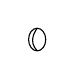
\begin{tikzpicture}[x=1ex,y=1ex,baseline=-.5ex]\draw (0,0) ellipse (.72 and .95);\draw (0,-.95) .. controls (-.75,-.15) and (-.2,.65) .. (0,.95);\end{tikzpicture}}}}\hand{\ensuremath{^{\wedge}}}, where
\hand{\ensuremath{\mathord{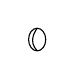
\begin{tikzpicture}[x=1ex,y=1ex,baseline=-.5ex]\draw (0,0) ellipse (.72 and .95);\draw (0,-.95) .. controls (-.75,-.15) and (-.2,.65) .. (0,.95);\end{tikzpicture}}}} is the category of ``\uline{standard he\over{mi}{mi}spheres}'', very similar to the catego-%
ries \hand{\ensuremath{\Delta}} and \hand{\ensuremath{\square}} of standard simplices resp. cubes, and even simpler than
these (being based on bigons, rather than \inserted{on} triangles or squares). In the
sequel, we often refer to this category \hand{\ensuremath{\mathord{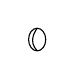
\begin{tikzpicture}[x=1ex,y=1ex,baseline=-.5ex]\draw (0,0) ellipse (.72 and .95);\draw (0,-.95) .. controls (-.75,-.15) and (-.2,.65) .. (0,.95);\end{tikzpicture}}}}, and to the ``trinity'' of the
three most beautiful ``test categories'' (in fact, they are even ``contrac-%
tors'')\hand{\ensuremath{\mathord{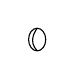
\begin{tikzpicture}[x=1ex,y=1ex,baseline=-.5ex]\draw (0,0) ellipse (.72 and .95);\draw (0,-.95) .. controls (-.75,-.15) and (-.2,.65) .. (0,.95);\end{tikzpicture}}}} ,\hand{\ensuremath{\Delta}} ,\hand{\ensuremath{\square}}, without having introduced formally \hand{\ensuremath{\mathord{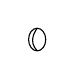
\begin{tikzpicture}[x=1ex,y=1ex,baseline=-.5ex]\draw (0,0) ellipse (.72 and .95);\draw (0,-.95) .. controls (-.75,-.15) and (-.2,.65) .. (0,.95);\end{tikzpicture}}}} anywhere in the
notes. \xout{As a matt} This category \hand{\ensuremath{\mathord{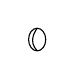
\begin{tikzpicture}[x=1ex,y=1ex,baseline=-.5ex]\draw (0,0) ellipse (.72 and .95);\draw (0,-.95) .. controls (-.75,-.15) and (-.2,.65) .. (0,.95);\end{tikzpicture}}}} has been first introduced in the the-%
sis of \uline{David} W. \uline{Jones} (a student of Ronnie Brown) ``\uline{Poly T-Complexes}'' ,
\xout{under the name of} and he calls the corresponding notion of complexes
``\uline{globular} complexes'' (instead of ``hemispherical''). That these do modeli-%
ze homotopy types, more accurately that \hand{\ensuremath{\mathord{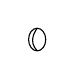
\begin{tikzpicture}[x=1ex,y=1ex,baseline=-.5ex]\draw (0,0) ellipse (.72 and .95);\draw (0,-.95) .. controls (-.75,-.15) and (-.2,.65) .. (0,.95);\end{tikzpicture}}}} is a (stric\over{\unsure{t}}{t}) test category,
will follow from the general criterion of section 31, much in the same
way as for\hand{\ensuremath{\Delta}} and \hand{\ensuremath{\square}}(see section 34 for these). It is clear that for the
study of stacks, hemispherical complexes will be better suited than
semisimplicial or cubical ones. It should'nt be hard anyhow to describe
functors going from one type of complexes to the other, in such a way \margin{\diagram{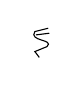
\begin{tikzpicture}[x=.8em,y=.7ex]\draw (.6,3)--(0,2.6) .. controls (-.3,1.4) and (.9,1.7) .. (.55,.8)--(0,.2)--(.2,-.5);\draw (.05,2.2)--(.65,2.4);\end{tikzpicture}}}

\mspage{\hand{89}}
